\graphicspath{{Chapters/Chapter_intro/}}

\chapter{Introduction}
\label{ch:intro}

Nuclear fusion is potentially a fantastic long-term energy source. On Earth, the fuel is abundant, the waste manageable, and is otherwise clean. The most easily accessible fusion reaction for us is the fusion of two heavy hydrogen isotopes: deuterium and tritium, with one and two neutron respectively. The reaction produces a neutron with 14.1 MeV of energy and a helium-4 nucleus with 3.5 MeV. In terms of mass of the reactants, the energy density of fusion is roughly seven orders of magnitudes higher than hydrocarbon fuels. Reaching the conditions for this fusion reaction requires of the plasma sufficiently high density $n$, temperature $T$, and confinement time $\tau$. Since the inception of the controlled fusion program, progress has been made towards improving these parameters \cite{wurzel_progress_2022}, but much work is left to be done to put the power of the sun in the palm of our hands.

\section{Nuclear fusion via magnetic confinement}

The current dominant structure for fusion plasmas is the donut-shaped tokamak \cite{john_wesson_tokamaks_2004}. This device operates by first imposing a toroidal field with external magnets, like bending a solenoid into a circle. Toroidal devices make intuitive sense: the magnetic field can only confine plasmas perpendicular to the field via the Lorentz force $F = q(E + v \times B)$, so the third axis is wrapped in a circle so that the magnetic field lines are closed. A current is induced in this toroidal direction to create an orthogonal poloidal field component, a net helical field, to cancel out particle drifts. As of this writing, tokamaks are in the lead for plasma performance in magnetic confinement fusion \cite{wurzel_progress_2022}.

Tokamaks, however, have two major drawbacks: the large toroidal current and the complicated geometry. At minimum, a breakeven reactor requires many millions of Amperes of circulating current \cite{creely_overview_2020}. This current is a source of free energy that, in situations called disruptions, can be dumped into an electron beam that causes catastrophic damage to the wall as well as structural damage via induced currents. These disruptions are thought by some to be a showstopper for the tokamak program, though personally, I am confident disruptions will be figured out given enough time and money. These disruptions can be avoided altogether by instead building a toroidal device that has a (mostly) externally set field. Such a device is called a stellarator \cite{boozer_what_1998}. These stellarators are, structurally speaking, even more complicated than a tokamak. The requirement for purely externally defined fields and sufficiently good confinement properties leads to very complicated coil geometries that are difficult and expensive to assemble. Devices that are difficult and expensive to build will not be economically competitive -- costs are very important to the viability of fusion reactors \cite{schwartz_value_2023}. Geometrically simple, linear devices, like mirror machines, may be the path forward despite intrinsically worse confinement. 

The magnetic mirror approach to fusion \cite{Post_1987} operates on the principle of conservation of the magnetic moment $\mu = \frac{W_\perp}{B}$. When a particle enters a region of higher field, $W_\perp$ increases by conservation of $\mu$. Given sufficiently high $W_\perp$ relative to $W_\parallel$, by conservation of energy ($W_\perp + W_\parallel = \text{constant}$) $W_\parallel$ must decrease and, on occasion, the particle must stop and reverse direction. Thus, some particle trapping can be achieved by creating a solenoid with two high field magnets at either end. Some particles can escape, and if the loss rate is rapid enough, deplete a portion of the velocity space leading to a ``loss cone'' distribution which can then drive many vicious instabilities. A schematic of this loss cone can be seen in fig. \ref{fig:loss-cone}. The primary focus of magnetic mirror research has been on plugging this hole in the distribution function and mitigating the interchange instability \cite{Post_1987}.

\begin{figure}
	\centering
	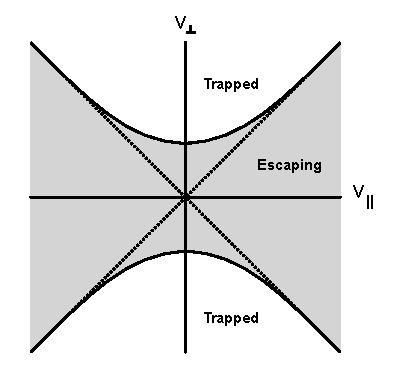
\includegraphics[width=230pt]{figures/loss-cone.pdf}
	\caption[The mirror machine loss cone]{\label{fig:loss-cone}Schematic of the velocity distribution loss cone in mirrors (for ions). Ions are lost for all perpendicular velocities below a certain threshold because of the ambipolar potential created by fast-escaping electrons.}
\end{figure}

\section{Confinement degradation from instabilities and turbulence}

All fusion plasmas are contained within a vacuum vessel and are hot relative to the vessel wall, which implies the existence of temperature and density (and thus pressure) gradients. These gradients provide free energy to drive instabilities, which in some cases cascade to smaller length scales and dissipate. This process is turbulence, and it occurs inside every fusion-relevant plasma that we know of. These turbulent eddies can be large and are the fundamental limit on cross-field transport for fusion reactors. Effort must be made to study and characterize this turbulence, and if possible, suppress it. 

Many instabilities contribute to transport and turbulence in fusion devices. Instabilities impact mirror machines will be briefly reviewed here. A detailed look at instabilities present in the LAPD can be found in chapters \ref{ch:background} and \ref{ch:mirror_turbulence}.

Drift waves are a common density gradient-driven instability, driven unstable by dissipation \cite{hendel_collisional_1968, Horton_1999, Tynan_review_2009}. These drift waves are commonly seen in magnetic confinement fusion devices given the minimal requirements of a density gradient and magnetic field. Other drift-like modes also exist, such as ion temperature gradient modes (ITG), trapped electron modes (TEM), and electron temperature gradient modes (ETG), summarized in Doyle 2007 \cite{physics_chapter_2007}.

Mirror machines have been primarily concerned with stabilization of flute-like interchange modes. These modes are driven by pressure gradients aligned with the magnetic field curvature vector \cite{Post_1987, ferron_interchange_1983, wickham_curvature-induced_1982}. These modes have been stabilized in a variety of ways, such as line-tying \cite{Fornaca_1979}, using a good-curvature expander tank \cite{Ryutov_2011,Ivanov_2013}, or non-axisymmetric magnetic field configurations \cite{moir_yin-yang_1969}. Ballooning modes \cite{dippolito_low-_1981} may also be driven unstable in mirror machines, and are commonly seen in tokamaks \cite{strait_stability_1994, connor_review_1998}.

Mirror machine research has also focused on velocity space instabilities driven by the loss cone distribution. The drift-cyclotron loss cone instability (DCLC) \cite{baldwin_potential-confined_1979, ferron_dependence_1984, kotelnikov_electrostatic_2017} is the coupling of ion drift waves to the ion cyclotron motion, driven by the density gradient and loss cone distribution. This mode can be stabilized by filling the loss cone, typically with warm plasma, so it is not expected to see this mode in a highly collisional plasma like the LAPD. The Alfv\'en ion cyclotron (AIC) instability is similar -- Alfv\'en waves interact with ion cyclotron motion, scattering the ions and degrading confinement \cite{Casper_1982}. 

\subsection{Importance of this turbulence and transport study}

As enumerated above, many instabilities may be present in a mirror machine, and understanding how modes may couple and influence transport is critical to design and operation of fusion reactors. Using the LAPD, we seek to understand turbulence and transport at edge-like conditions of mirror machines, and attempt to observe the interaction of interchange modes with drift waves or other instabilities. This study also highlights the ability for the LAPD to operate with mirror configurations, which may be useful for future studies since mirrors are once again being considered for a fusion reactor \cite{WHAM, BEAM, frank_integrated_2024}. In addition, characterization of modes present on the LAPD would give a greater understanding in interpreting data in other LAPD studies. Disentangling or enumerating possible modes present could illuminate promising directions for further studies on LAPD turbulence and transport.

The magnetic field of the LAPD was configured to create several mirror ratios and lengths, with focus primarily on short mirror cases. These mirrors were diagnosed with Langmuir probes and magnetic probes. Spectra from these diagnostics were analyzed to determine the modes present and calculate cross-field particle flux. Additional data were collected to reconstruct the 2d structure of the modes present using correlation techniques. Drift-Alfv\'en waves were observed at 12 kHz and up with the peak having strong dependence on machine-averaged magnetic field, as expected. Lower frequency modes could not be confidently identified, and could be a mixture of drift waves, rotational interchange, a nonlinear instability, or the conducting wall mode. Particle flux measurements were unexpected: with increased mirror ratio, the particle flux decreased. Magnetic curvature has a destabilizing effect, so an increased $E \times B$ particle flux was expected. Nevertheless the particle diffusivity estimate was consistent with Bohm diffusion. The decrease in particle flux could be explained in-part but the decrease gradient scale length caused by the larger plasma radius at higher mirror ratios. No evidence for the interchange mode was observed, likely because of many stabilization methods present.

Although the results are unexpected, they are promising when considering the cold edge of a fusion reactor. If the edge is in contact with a conducting surface, it will likely be stable and not contribute too greatly beyond typical Bohm (or turbulent) transport. 

\section{Accelerating research using machine learning}

Machine learning, though a nascent field for quite some time, has exploded in popularity since the advent of deep neural networks trained on GPUs \cite{krizhevsky_imagenet_2017}. Machine learning is effectively curve fitting, though, as compute is becoming cheaper and GPUs more powerful, larger models can be trained with greater capabilities. Fundamentally, machine learning, and in particular deep learning, scale very well with data and dimensionality. Plasma devices collect a significant amount of data and so do the simulations used to interpret the experimental data.

Recently, machine learning techniques have become increasingly used in the plasma physics and nuclear fusion community. 
One of the most common applications is building surrogate models for expensive simulations. Surrogates train on simulation output and, once learned, provide a fast way enable fast predictions in the domain covered by the training set. Surrogate modeling \cite{taylor_how_2021} has been applied to turbulence and transport computations \cite{meneghini_neural-network_nodate,li_surrogate_2025,fransson_fast_2023,ho_neural_2021}, profile prediction \cite{morosohk_realtime_2023}, global tokamak simulations \cite{dong_deep_2021}, uncertainty quantification \cite{yudin_uncertainty_2024}, and in inertial confinement fusion (ICF) \cite{nora_ensemble_2017, anirudh_improved_2019}. ICF in particular has had great success incorporating experimental data into theoretical models using machine learning to enhance their predictive capabilities  \cite{gaffney_making_2019, humbird_cognitive_2021, gopalaswamy_tripled_2019}.

Reinforcement learning has been used for trajectory control on tokamaks \cite{seo_feedforward_2021, seo_development_2022, seo_avoiding_2024}, notably on the TCV tokamak \cite{degrave_magnetic_2022,tracey_towards_2024} for exploring new magnetic configurations. Predicting instabilities, particularly disruptions, has also been a major application of machine learning in the field \cite{rea_real-time_2019, kates-harbeck_predicting_2019, pau_machine_2019,fu_machine_2020, murari_investigating_2020, rea_progress_2020, rossi_hybrid_2024}. A comprehensive review of disruption prediction can be seen in Vega et al. \cite{vega_disruption_2022}. 

Profile prediction in tokamaks has also been performed using machine learning. Electron density, temperature, and other quantities in tokamaks have been predicted \cite{abbate_data-driven_2021, dong_machine_2021}, and can be adaptable using reservoir NNs  \cite{jalalvand_real-time_2022}. Temporal evolution of parameters has been successfully modeled using recurrent neural networks (RNNs)\cite{char_full_2024, wan_east_2022, seo_feedforward_2021, seo_development_2022}.

Machine learning techniques can also be used to solve differential equations by parameterizing the solution using a neural network. These ``physics-informed neural networks'' (PINNs) have also been increasingly used in fusion \cite{rossi_potential_2023, aymerich_physics_2023, seo_leveraging_2024}.

A deeper review of machine learning with respect to profile prediction and generative modeling can be found in chapters \ref{ch:isat-predict} and \ref{ch:ebm}, respectively.

\subsection{Importance of these ML models}

The study of plasmas is characterized by temperamental experiments, incomplete and untrustworthy diagnostics, and difficult theory. Machine learning provides a new tool to tackle these challenges. As demonstrated in the referenced works above, machine learning can be used to great effect to accelerate simulations, control plasmas, and make predictions. In order to successfully accomplish these tasks, these models learn some structure (such as a lower-dimensional manifold) over the data, but this structure is usually exploited only for the downstream task, such as predicting a plasma parameter at some point in time or an actuator state. My goal is to make this structure explicit and explorable; the model has likely learned relationships that can improve our understanding of fusion plasmas. If a model learns relevant and useful relationships from data, then this information can be exploited without requiring painstaking manual data analysis, dramatically accelerating the rate of progress in fusion science.

This work pushes the frontier of extracting insight from a plasma device using machine learning. A diverse set of machine configurations were collected on the Large Plasma Device (LAPD) sampling from machine settings using Latin hypercube sampling. This randomization of machine configurations is a first for magnetized plasma research and yielded a set of 44 randomized dataruns (67 dataruns in total) spanning a wide range of LAPD parameter space, totalling 132,000 discharges. The diversity of this dataset is unique for plasma physics research: usually most machine parameters are held constant and vary one or a few in a grid-like pattern, but here all parameters are changed. 

Using a small neural network (around 200,000 parameters), time-averaged ion saturation current ($I_\text{sat}$) can be predicted at virtually any point in the Large Plasma Device (LAPD) given the machine state. Information is extracted from this model by inferring trends: scanning along particular inputs and observing how the predicted $I_\text{sat}$ changes. Trends inferred this way agree with intuition and arguments from geometry, demonstrating that the model has accurately learned the underlying relationships. In addition, this model is used to optimize the axial variation of $I_\text{sat}$ in LAPD discharges. Axial variation in density and temperature is an important problem affecting many physics studies on the LAPD and the ability to optimize the axial variation can alleviate this issue. Machine learning is required to perform this trend inference and optimization of LAPD plasmas: the dimensionality of the problem is too high for a conventional grid search. Fundamentally, this work demonstrates the new capability of searching a high-dimensional space on a plasma device that would be very difficult, if impossible, to do without machine learning.

This work was extended to additional diagnostics and time-series data, and expanded to generative modeling. An energy-based model (EBM) was trained on these additional diagnostics, learning a joint distribution over the diagnostics and machine parameters. This model can be used to reconstruct diagnostics signals given any combination of inputs. In this case the interferometer signal was inferred from only machine parameters as well as including additional diagnostic signals. Additional, unanalyzed and uncalibrated, signals improved reconstruction performance, indicating that other diagnostics contain useful information even in a primitive form. This diagnostic reconstruction using generative modeling is a first for plasma science, and this reconstruction was performed by modifying the energy function in a novel way. In addition, the energy surface was directly examined by scanning along the probe x-axis dimension, demonstrating a novel ability to find symmetries in the data from the trained model. These EBMs provide a very flexible way of representing the data, and open up many possibilities for combining with additional datasets and simulations.

Fundamentally, the machine learning techniques demonstrated in this thesis provide a pathway towards automating fusion science, and demonstrates a new way of representing and analyzing data over a wide range of experimental conditions. 

\section{Outline of the dissertation}
Chapter \ref{ch:background} describes the Large Plasma Device, the configuration of the machine, and the diagnostics used in this thesis. It also provides background on some relevant instabilities and a very brief introduction to neural networks. 

Chapter \ref{ch:mirror_turbulence} details a study of mirror turbulence and transport using the older barium oxide cathode. Multiple mirror ratios and lengths were analyzed, with the conclusion being that cross-field particle flux reduced at higher mirror ratios, and no evidence of the interchange instability was seen.

Chapter \ref{ch:ml-dataruns} describes the process of collecting data from randomly-set LAPD configurations, the diagnostics collected, and the biases inherent in the data. The dataset collected here is used in the two subsequent chapters. The chapter also covers the data cleaning process for some of the diagnostics. 

Chapter \ref{ch:isat-predict} is a thorough machine learning study on predicting ion saturation current -- $I_\text{sat}$ -- in LAPD mirrors using neural networks. This is possibly the first time a global optimization like this has been performed in magnetized plasma device. In addition, trends were inferred by scanning along various combinations of machine inputs. The important features of this work are the validation of model predictions and thorough uncertainty quantification. Fundamentally, this is a demonstration that machine learning can be used to extract insights from data in a complicated, multivariate physical system. 

Chapter \ref{ch:ebm} takes a different angle on machine learning than what was done in chapter \ref{ch:isat-predict}. Instead of predicting a single output given machine inputs, we instead learn a probability distribution over the data using an energy-based model. Using this model, we can reconstruct any arbitrary combination of diagnostics, machine settings, or anything in the input space -- including hallucinating discharges altogether. The flexibility of the learned energy function is demonstrated, and this flexibility may be a way to combine theory and experiment to improve predictions. 

Appendix \ref{app:0d-mirror} describes a small 0d reactor optimization project in collaboration with Kunal Sanwalka, based on a spreadsheet by Cary Forest. This project was undertaken to learn how to use Jax and SymPy, and also gain some intuition on mirror-based fusion reactors.
